\documentclass[12pt]{article}

\usepackage[letterpaper, margin=1.0in]{geometry}
\usepackage{appendix}
\usepackage[utf8]{inputenc}
\usepackage[T1]{fontenc}
\usepackage{siunitx}
\usepackage{caption}
\usepackage{moreverb}
\usepackage{parskip}
\usepackage{multirow}
\usepackage{adjustbox}
\usepackage{enumerate}
\usepackage{listings}
\usepackage{graphicx}
\usepackage{pdfpages}
\usepackage[american,straightlabels]{circuitikz}
\usepackage{fancyhdr}
\usepackage[explicit]{titlesec}
\usepackage{xcolor}
\usepackage[many]{tcolorbox}
\usepackage{eqparbox}
\usepackage{hyperref}
\usepackage{listings}

\lstdefinelanguage[mips]{Assembler}{%
  % so listings can detect directives and register names
  alsoletter={.\$},
  % strings, characters, and comments
  morestring=[b]",
  morestring=[b]',
  morecomment=[l]\#,
  % instructions
  morekeywords={[1]abs,abs.d,abs.s,add,add.d,add.s,addi,addiu,addu,%
    and,andi,b,bc1f,bc1t,beq,beqz,bge,bgeu,bgez,bgezal,bgt,bgtu,%
    bgtz,ble,bleu,blez,blt,bltu,bltz,bltzal,bne,bnez,break,c.eq.d,%
    c.eq.s,c.le.d,c.le.s,c.lt.d,c.lt.s,ceil.w.d,ceil.w.s,clo,clz,%
    cvt.d.s,cvt.d.w,cvt.s.d,cvt.s.w,cvt.w.d,cvt.w.s,div,div.d,div.s,%
    divu,eret,floor.w.d,floor.w.s,j,jal,jalr,jr,l.d,l.s,la,lb,lbu,%
    ld,ldc1,lh,lhu,li,ll,lui,lw,lwc1,lwl,lwr,madd,maddu,mfc0,mfc1,%
    mfc1.d,mfhi,mflo,mov.d,mov.s,move,movf,movf.d,movf.s,movn,movn.d,%
    movn.s,movt,movt.d,movt.s,movz,movz.d,movz.s,msub,msubu,mtc0,mtc1,%
    mtc1.d,mthi,mtlo,mul,mul.d,mul.s,mulo,mulou,mult,multu,mulu,neg,%
    neg.d,neg.s,negu,nop,nor,not,or,ori,rem,remu,rol,ror,round.w.d,%
    round.w.s,s.d,s.s,sb,sc,sd,sdc1,seq,sge,sgeu,sgt,sgtu,sh,sle,%
    sleu,sll,sllv,slt,slti,sltiu,sltu,sne,sqrt.d,sqrt.s,sra,srav,srl,%
    srlv,sub,sub.d,sub.s,subi,subiu,subu,sw,swc1,swl,swr,syscall,teq,%
    teqi,tge,tgei,tgeiu,tgeu,tlt,tlti,tltiu,tltu,tne,tnei,trunc.w.d,%
    trunc.w.s,ulh,ulhu,ulw,ush,usw,xor,xori,setx,bex},
  % assembler directives
  morekeywords={[2].align,.ascii,.asciiz,.byte,.data,.double,.extern,%
    .float,.globl,.half,.kdata,.ktext,.set,.space,.text,.word},
  % register names
  morekeywords={[3]\$0,\$1,\$2,\$3,\$4,\$5,\$6,\$7,\$8,\$9,\$10,\$11,%
    \$12,\$13,\$14,\$15,\$16,\$17,\$18,\$19,\$20,\$21,\$22,\$23,\$24,%
    \$25,\$26,\$27,\$28,\$29,\$30,\$31,%
    \$zero,\$at,\$v0,\$v1,\$a0,\$a1,\$a2,\$a3,\$t0,\$t1,\$t2,\$t3,\$t4,
    \$t5,\$t6,\$t7,\$s0,\$s1,\$s2,\$s3,\$s4,\$s5,\$s6,\$s7,\$t8,\$t9,%
    \$k0,\$k1,\$gp,\$sp,\$fp,\$ra},
}[strings,comments,keywords]

\lstdefinestyle{myVerilog}{
  language=Verilog,
  basicstyle=\tiny,
  frame=shadowbox,                    
  rulesepcolor=\color{blue}
}

\lstdefinestyle{myMips}{
  language=[mips]Assembler,
  basicstyle=\tiny,
  frame=shadowbox,                    
  rulesepcolor=\color{blue}
}

\hypersetup{
    colorlinks=true,
    linkcolor=black,
    filecolor=magenta,      
    urlcolor=blue,
}

\pagestyle{fancy}

\renewcommand{\headrulewidth}{0.2mm}
\renewcommand{\footrulewidth}{0.2mm}

\fancyhead[L]{ECE 350}
\fancyhead[R]{Page \thepage}
\fancyfoot[L]{Final Project}
\fancyfoot[C]{Carreiro, Yaras}
\fancyfoot[R]{Page \thepage}

\def\arraystretch{1.5}

\begin{document}
\title{ECE 350 Final Project}
\author{Januario Carreiro and John Yaras}
\date{\today}

\maketitle

\thispagestyle{fancy}

\newpage

\section{Project Design and Specifications}
For the final project, we decided to build and implement an {\tt XY-Plotter}, which is a device that can guide a pen along two axes in order to create an image on a piece of paper. For the hardware, we settled on the SUNWIN Laser Engraving Machine as a starting point. This kit included the mechanisms necessary to draw on two axes, and we would go on to add a mechanism to lift and lower our writing instrument.

\begin{table}[ht!]
\centering
\begin{tabular}{|c|c|} \hline
Part & Quantity \\ \hline \hline
Acrylic Shelf & 8 \\ \hline
Aluminum Beams & 4 \\ \hline
Aluminum Guideway & 1 \\ \hline
Ball Bearing & 13 \\ \hline
Flat Washer & 12 \\ \hline
Hex Nut & 20 \\ \hline
Hex Screw & 28 \\ \hline
Phillips Screw & 36 \\ \hline
Plastic Washer & 20 \\ \hline
Servo Motor & 1 \\ \hline
Sharpie & 1 \\ \hline
Stepper Motor & 2 \\ \hline
T Nut & 8 \\ \hline
\end{tabular}
\caption{Parts List for Plotter}
\end{table}

The plotter itself is primarily made from aluminum beams, acrylic shelves, and metal screws. Each motor is placed on a different acrylic shelf and secured with metal screws. The mechanism for moving the writing instrument is a wheel and track: as the servo motors spin, the friction between the sprockets on the wheels placed on the servo motor and the track cause the acrylic shelf on which the writing instrument is placed to be moved.

While the writing surface is 40 cm x 50 cm, the reachable area is only 35 cm x 45 cm. This is due the nature of the pen raise/lower mechanism: the pen is raised and lowered with a servo motor and is always at a tilt---the protrusion of the pen decreases the available writing area. Furthermore, the reachable area can possibly be less than 35 cm x 45 cm depending on the surface on which the plotter is placed: it requires a perfectly flat surface. If the plotter were to placed on a surface with substantive cavities, the pen would lose contact with the surface and the drawing will not complete as desired.

\section{Input and Output}
To give instructions to the FPGA, a system similar to Logo's turtle graphics module was implemented with the following format:

\begin{figure}[ht!]
\centering
\begin{tabular}{|c|c|c|c|} \hline
OP & H2 & H1 & H0 \\ \hline
\multicolumn{1}{c}{} & \multicolumn{3}{p{2cm}}{\raisebox{.5\baselineskip}{$\underbrace{\hspace{2.45cm}}$}} \\
\multicolumn{1}{c}{} & \multicolumn{3}{c}{Hex Digits} \\
\end{tabular}
\caption{Instruction Format}
\end{figure}

Here, {\tt OP} is an ascii character code for either {\tt F, L} or {\tt R}. If {\tt OP} is {\tt F} then the digits that follow are interpreted as a number of rotations of the stepper motor. If {\tt OP} is instead {\tt L} or {\tt R}, then the digits that follow are interpreted as degrees. This system where the pen moves with commands relative to its own position was chosen for two reasons: (1) the stepper motors and the tracks slowly decalibrate as they move, so a coordinate system would provide wonky images, and (2) turtle geometry has a short learning curve: anyone can easily control {\tt XY-Plotter} with minimal instruction---after all, Logo was designed as an educational programming language.

The input is transmitted from the Raspberry Pi to the FPGA via the Universal Asynchronous Receiver/Transmitter (UART) serial interface by way of the {\tt TX} pin. As each character is transmitted from the Raspberry Pi GPIO interface to the FPGA GPIO interface, the character is placed directly into the DMEM module of the processor. An END character designated as ``11'' in ASCII marks the end of the instruction and the beginning of the processor operation. Below, we include the Verilog code for the UART DMEM module:

\begin{lstlisting}[style=myVerilog, caption={The UART DMEM Interface}]
module uart_wrapper(input clk, input rx, input wren, input [11:0] address_dmem, input [31:0] data, 
	output [31:0] q_dmem, output reg done);

	wire data_ready;
	wire [7:0] uart_q;
	
	reg [7:0] delay;
	reg [11:0] index;
	
	initial begin
		done <= 0;
		index <= 12'b0;
		delay <= 8'b0;
	end

	always @(posedge data_ready) begin
		index <= (uart_q == 8'd10) ? 12'b0 : index + 1;
		if (uart_q == 8'd11)
			delay <= 1;
		else if (uart_q == 8'd10)
			delay <= 0;
	end
	
	always @(posedge clk) begin
			if (delay == 1)
				done <= 1;
			else if (delay == 0)
				done <= 0;
	end
	
	uart_rx receiver(clk, rx, data_ready, uart_q);
	dmem my_dmem(done ? address_dmem : index, ~clk, done ? q_dmem : {24'b0, uart_q}, 
		done ? wren : data_ready, q_dmem);
endmodule
\end{lstlisting}

In the processor, there are certain registers which are responsible for determining the duty cycle for the servo motor. The PWM wave to control the servo motor is generated with period 20 ms and duty cycle specified by a constant driven by the value in register {\tt R6}. The PWM duty cycle determines the angle the servo motor is set to. A diagram of the inputs to the Servo Motor is given below:

\begin{figure}[ht!]
\begin{center}
\begin{circuitikz}
\ctikzset{multipoles/thickness=3}
\ctikzset{multipoles/dipchip/width=2}
\draw (0,0) node[dipchip, num pins=6, hide numbers, no topmark, external pins width=0](C){};
\node [right, font=\tiny] at (C.bpin 1) {SIGNAL};
\node [right, font=\tiny] at (C.bpin 2) {VCC};
\node [right, font=\tiny] at (C.bpin 3) {GND};
\draw (C.bpin 1) 	to[short, -o] ++ (-1,0) node[anchor=east] {GPIO 21};
\draw (C.bpin 2) 	to[short, -o] ++ (-1,0) node[anchor=east] {5V};
\draw (C.bpin 3) 	to[short, -o] ++ (-1,0) node[anchor=east] {GND}; 
\end{circuitikz}
\end{center}
\caption{Circuit Diagram for Servo Motor}
\end{figure}

The outputs from the processor are transmitted to Servo Motor for controlling pen elevation. Here, we include the Verilog code for the Servo Motor driver:

\begin{lstlisting}[style=myVerilog, caption={The Servo Motor Controller}]
module servo_controller(input clk, input [31:0] counter_limit, output reg pwm);
	reg [31:0] counter;
	
	initial begin
		pwm <= 0;
		counter <= 32'b0;
	end
	
	always @(posedge clk) begin
		if (0 <= counter && counter <= counter_limit) begin
			pwm <= 1;
			counter <= counter + 1;
		end else if (counter_limit < counter && counter <= 1000000) begin
			pwm <= 0;
			counter <= counter + 1;
		end else begin
			counter <= 32'b0;
		end
	end
endmodule
\end{lstlisting}

While the output of the FPGA can be directly transmitted to the servo motor, communicating with the stepper motors is more difficult and is done through drivers. This is because the stepper motors require a lot more voltage and current than the servo motors: while the servo operates at 5 V, the stepper motors often pull 13 V and 0.5 mA. To communicate with the drivers, there are certain registers which are responsible for determining the step counter and direction. These parameters drive the step clock which in turn affects the speed of the motors. The Verilog code for the Stepper Motor controller is given below:

\begin{lstlisting}[style=myVerilog, caption={The Stepper Motor Controller}]
module stepper_controller(input clk, input enable, input [31:0] counter_limit, output reg step_clk);
	reg [31:0] step_counter;
	
	initial begin
		step_clk <= 1'b0;
		step_counter <= 32'b0;
	end
	
	always @(posedge clk) begin
		if (enable && counter_limit != 32'b0) begin
			step_counter <= step_counter + 1;
		end
		
		if (step_counter >= counter_limit) begin
			step_clk <= ~step_clk;
			step_counter <= 32'b0;
		end
	end
endmodule
\end{lstlisting}

We also include a diagram of the the inputs and outputs of the Stepper Motor Drivers:

\begin{figure}[ht!]
\begin{center}
\begin{circuitikz}
\ctikzset{multipoles/thickness=3}
\ctikzset{multipoles/dipchip/width=2}
\draw (0,0) node[dipchip, num pins=16, hide numbers, no topmark, external pins width=0](C){};
\node [right, font=\tiny] at (C.bpin 1) {ENABLE};
\node [right, font=\tiny] at (C.bpin 2) {M0};
\node [right, font=\tiny] at (C.bpin 3) {M1};
\node [right, font=\tiny] at (C.bpin 4) {M2};
\node [right, font=\tiny] at (C.bpin 5) {RESET};
\node [right, font=\tiny] at (C.bpin 6) {SLEEP};
\node [right, font=\tiny] at (C.bpin 7) {STEP};
\node [right, font=\tiny] at (C.bpin 8) {DIR};
\node [left, font=\tiny] at (C.bpin 16) {VMOT};
\node [left, font=\tiny] at (C.bpin 15) {GND};
\node [left, font=\tiny] at (C.bpin 14) {B2};
\node [left, font=\tiny] at (C.bpin 13) {B1};
\node [left, font=\tiny] at (C.bpin 12) {A1};
\node [left, font=\tiny] at (C.bpin 11) {A2};
\node [left, font=\tiny] at (C.bpin 10) {VDD};
\node [left, font=\tiny] at (C.bpin 9) {GND};
\draw (C.bpin 5) 	to[short] ++ (-1,0) node(n1) {};
\draw (C.bpin 6) 	to[short] ++ (-1,0) 
					to[short] (n1);
\draw (C.bpin 7) 	to[short, -o] ++ (-2,0) node[anchor=east] {GPIO 13}; % UPDATE
\draw (C.bpin 8) 	to[short, -o] ++ (-2,0) node[anchor=east] {GPIO 15}; % UPDATE
\draw (C.bpin 9) 	to[short] ++ (1,0) 
					to[short] ++ (0,-1) node(n2) {}
					to[short] (n2 -| n1) 
					to[short, -o] ++(-1,0) node[anchor=east] {3.3V}; % UPDATE
\draw (C.bpin 10) 	to[short] ++ (1.6,0) node(n3) {}
					to[short] (n3 |- n2)
					to[short] ++(0,-.6) node(n4) {}
					to[short] (n4 -| n1) 
					to[short, -o] ++(-1,0) node[anchor=east] {GND}; % UPDATE
\draw (C.bpin 11) 	to[short, -o] ++ (2,0) node[anchor=west] {PHASE /A};
\draw (C.bpin 12) 	to[short, -o] ++ (2,0) node[anchor=west] {PHASE A};
\draw (C.bpin 13) 	to[short, -o] ++ (2,0) node[anchor=west] {PHASE /B};
\draw (C.bpin 14) 	to[short, -o] ++ (2,0) node[anchor=west] {PHASE B};
\draw (C.bpin 15) 	to[short] ++ (4,0) 
					to[short] ++ (0,2) node(n5) {}
					to[short, -o] ++ (0,1) node[anchor=south] {GND};
\draw (C.bpin 16) 	to[short] ++ (2,0) node(n6) {}
					to[short] (n6 |- n5) node(n7) {}
					to[C, l_=\SI{47}{\nano\farad}] (n5);
\draw (n7)			to[short, -o] ++(0,1) node[anchor=south] {VDD};
\end{circuitikz}
\end{center}
\caption{Circuit Diagram for Stepper Motor Drivers}
\end{figure}

As you can see from the diagram, the process of communicating with the stepper motors is a lot more involved. And, due to the instant changes in voltage and current required from the stepper motors as they change speed and direction, a capacitor is required between VDD and ground as to not damage the driver.

Having shown the inputs to the motors (which include GPIO pins found on the FPGA), we include a diagram of all of the inputs and outputs to the FPGA for completeness:

\begin{figure}[ht!]
\begin{center}
\begin{circuitikz}
\ctikzset{multipoles/thickness=3}
\ctikzset{multipoles/dipchip/width=2}
\draw (0,0) node[dipchip, num pins=12, hide numbers, no topmark, external pins width=0](C){FPGA};
\node [left, font=\tiny] at (C.bpin 12) {GPIO 11};
\node [left, font=\tiny] at (C.bpin 11) {GPIO 13};
\node [left, font=\tiny] at (C.bpin 10) {GPIO 15};
\node [left, font=\tiny] at (C.bpin 9) {GPIO 17};
\node [left, font=\tiny] at (C.bpin 8) {GPIO 19};
\node [left, font=\tiny] at (C.bpin 7) {GPIO 21};
\draw (C.bpin 7) 	to[short, -o] ++ (1,0) node[anchor=west] {Servo};
\draw (C.bpin 8) 	to[short, -o] ++ (1,0) node[anchor=west] {Y Dir};
\draw (C.bpin 9) 	to[short, -o] ++ (1,0) node[anchor=west] {Y Step}; 
\draw (C.bpin 10) 	to[short, -o] ++ (1,0) node[anchor=west] {X Dir};
\draw (C.bpin 11) 	to[short, -o] ++ (1,0) node[anchor=west] {X Step};
\draw (C.bpin 12) 	to[short, -o] ++ (1,0) node[anchor=west] {TX};
\end{circuitikz}
\caption{Circuit Diagram for FPGA Inputs and Outputs}
\end{center}
\end{figure}

Lastly, we will mention one other output: the Seven Segment Displays on the FPGA. These are used to specify the current instruction and were also extensively used for debugging purposes. 

\section{Changes to Processor}
Several changes were made to the processor. The first changes made were exposing the registers that changed relevant parameters for motor operation such as step size and direction.

Another change was adding support for a custom turtle-graphics-like language we designed for communicating with the Raspberry Pi and the motors.

Lastly, we also used stalls in the assembly code to let each line be drawn for the correct duration. This was done by setting a counter limit and incrementing the counter by one until it hit the correct value. This action tricked the FPGA into stalling for the exact time necessary and was reliant on the fact that the FPGA had a 50 MHz clock. Different counter limits would have had to have been calculated using Equation (1) if the speed of the motors and frequency of the FPGA had been different.

Otherwise, the only addition to the processor that would have been useful would have been the capability to do floating point math. However, adding support for floating points was deemed to be an irresponsible use of time given the time constraints, so we used a system of lookup tables (with significant multipliers) inserted into the DMEM in order to get around the need for floating point math.

\section{Challenges Faced}
Implementing the UART was challenging for several reasons. First, slowing down the clock of the FPGA to match the BAUD rate of the transmitting Raspberry Pi proved to be difficult since the BAUD rate is 9600 and does not divide evenly into a 50 MHz clock. Second, each bit some time to settle which meant reading them too early would produce an incorrect reading and reading too late would cause the bit to be missed because at that point a new bit would have already have been transmitted from the Raspberry Pi. Finally, it was also difficult to transfer control from the UART module to the processor when reading was done because the last bit would be writing as the reset on the processor was released which caused several timing issues that were difficult to both find and resolve.

Another challenge was what we call the division problem. The formula for determining the speed at which each motor would operate involved dividing the distance determined

In order to finely control the speed of each motor, we needed to find the so-called counter limit which determines when the step clock signal should change parity. The formula for this constant is given by
\begin{align}
\mbox{Counter Limit} = \frac{f_C}{2 f_M}
\end{align}
where $f_C$ is the clock frequency of the FPGA and $f_M$ is the desired rotational frequency of the stepper motor. This was problematic because it required doing division, which could take a long time in the processor. To solve the issue, we manually calculated stepper counter values and stored them in data memory. Whenever the processor required the value for a certain stepper counter, it could look them up in data memory, which only took one cycle as opposed to the 64 it would have been required had the processor had to do division.

Another challenge involved generating the instructions to be sent to the plotter. Initially, we used an Arduino as the transmitter to the FPGA but soon realized that it was difficult to replace the instructions on the Arduino as easily and quickly as we wanted to, for we wanted to provide an interface where one could provide pseudo-turtle code and instantly see the result. For this reason, we replaced the Arduino with a Raspberry Pi and then used the Raspberry Pi's GPIO pins to send instructions to the FPGA, which would instantly process them and send them along to the plotter.

\section{Testing}
The first thing that was tested was the stepper motor. Since neither of us had ever worked with stepper motors before, we quickly prototyped a circuit using a breadboard, wrote some Arduino code, and messed around with the Stepper motor until we could understand how to communicate with it effectively. 

After making sure the stepper motors worked on their own, we built the base of the {\tt XY-Plotter} and plopped the stepper motors in position. Then, using the Arduino code and circuit from before, we tested the stepper motors on the base to make sure that the tracks were moving properly.

Once we were sure the stepper motors and the tracks were working as expected, we moved on to trying to communicate with the stepper motors using the FPGA. At first, we wanted to communicate directly from the FPGA to the stepper motors, but we soon realized that a better design would be using the Arduino as a buffer between the FPGA and the stepper motors. This way, we could have the FPGA working to decode and interpret instructions as soon as they were received and send the decoded instructions to the Arduino without any need for stalling. The Arduino's built-in serial buffer could then be used as a queue of instructions for the the Arduino to convert to stepper motor movement without much hassle.

However, as we alluded to in the Challenges Faced section, the Arduino was not providing the performance that we were looking for. As such, we decided to move on from the Arduino and to a Raspberry Pi. One of the benefits of this is that it also made the project more portable: no longer would a laptop be required for transmitting messages---the Raspberry Pi can create and transmit whatever instructions we want.

Even though using the Raspberry Pi was a big improvement on the Arduino, getting everything to work properly was still a slow process. To speed up the error correction and error detection, we began to use the Seven Segment Displays on the FPGA. A big problem we were having is that we were not sure whether each instruction was being correctly transmitted to the FPGA and then added to DMEM---and there was no easy way to check until we started using the seven segment displays. Being able to see exactly what was being sent between the Raspberry Pi and the FPGA saved countless hours that would have been spent debugging. The code for the display is included below:

\begin{lstlisting}[style=myVerilog, caption={ASCII on Seven Segment Display}]
module ascii_to_display(clk, in, out);
	input clk;
	input [7:0] in;
	output reg [6:0] out;
	
	always @(posedge clk) begin
		case (in)
			8'd102 : out <= ~7'b1000111; // f (forward)
			8'd114 : out <= ~7'b0000101; // r (right)
			8'd108 : out <= ~7'b0001110; // l (left)
			8'd117 : out <= ~7'b0111110; // u (up)
			8'd100 : out <= ~7'b0111101; // d (down)
			8'd0   : out <= ~7'h7E; 	  // 0
			8'd1   : out <= ~7'h30;      // 1
			8'd2   : out <= ~7'h6D;      // 2
			8'd3   : out <= ~7'h79;      // 3
			8'd4   : out <= ~7'h33;      // 4
			8'd5   : out <= ~7'h5B;      // 5
			8'd6   : out <= ~7'h5F;      // 6
			8'd7   : out <= ~7'h70;      // 7
			8'd8   : out <= ~7'h7F;      // 8
			8'd9   : out <= ~7'h7B;      // 9
			default : out <= ~7'b1001111; // E
		endcase
	end
endmodule
\end{lstlisting}

\section{Possible Improvements/Features}
One quality-of-life improvement would be the addition of sensors to detect when the plotter moves too close to the edges. Right now, we manually take care of making sure that the writing instrument is always close to the center of plotter---if it reaches the edge then the force of the stepper motors would damage the writing instrument. If we added four pairs of sensors (one for each end of each axis), then we would be able to even run the plotter autonomously as there would be no worries about the plotter damaging itself while it ran. 

While adding sensors would certainly be a great improvement, the most important improvement would be adding the ability for the pen to move and down directly. As of now, we move the pen up and down on a swivel, and even though this does add the important ability to move around without drawing on the paper, when the pen is being used to draw it can sometimes either not have enough pressure or have too much pressure. If we had the ability to move the pen up and down directly, the pen would not have more or less pressure placed on it based on the direction its moving---pressure would be placed evenly on every direction. This would add stability to the pen and almost definitely improve accuracy.

Finally, a significant improvement to efficiency could be had by packing each instruction into a single word. As of now, each instruction takes up 4 words. However, each part of the instruction is only 8 bits long. Thus, it would definitely be possibly to create a much more compact storage scheme (in fact, four times more compact) which would then greatly improve our capacity to draw complicated images. 

\newpage
\section{Code}
\begin{lstlisting}[style=myVerilog, caption={The Top Level Module}]
module plotter_machine(input clk, input rx, input switch,
	output [0:6] h3, output [0:6] h2, output [0:6] h1, output [0:6] h0, 
	output reset, output x_step_clk, output x_dir, output y_step_clk, output y_dir, 
	output error, output pwm);

	processor(
	    clk,                            // I: The master clock
	    reset,                          // I: A reset signal
	    
	    address_imem,                   // O: The address of the data to get from imem
	    q_imem,                         // I: The data from imem
	
	    address_dmem,                   // O: The address of the data to get or put from/to dmem
	    data,                           // O: The data to write to dmem
	    wren,                           // O: Write enable for dmem
	    q_dmem,                         // I: The data from dmem
	
	    ctrl_writeEnable,               // O: Write enable for regfile
	    ctrl_writeReg,                  // O: Register to write to in regfile
	    ctrl_readRegA,                  // O: Register to read from port A of regfile
	    ctrl_readRegB,                  // O: Register to read from port B of regfile
	    data_writeReg,                  // O: Data to write to for regfile
	    data_readRegA,                  // I: Data from port A of regfile
	    data_readRegB,                  // I: Data from port B of regfile
	);
	
	wire done;
	assign reset = ~done;
	
	wire [11:0] address_dmem;
	wire [31:0] data;
	wire wren;
	wire [31:0] q_dmem;
	
	uart_wrapper (clk, rx, wren, address_dmem, data, q_dmem, done);
	
	wire [11:0] address_imem;
	wire [31:0] q_imem;
	
	imem my_imem(
	    .address    (address_imem),            // address of data
	    .clock      (~clk),                    // you may need to invert the clock
	    .q          (q_imem)                   // the raw instruction
	);
	 
	wire ctrl_writeEnable;
	wire [4:0] ctrl_writeReg, ctrl_readRegA, ctrl_readRegB;
	wire [31:0] data_writeReg;
	wire [31:0] data_readRegA, data_readRegB;
	regfile my_regfile(
	    clk,
	    ctrl_writeEnable,
	    reset,
	    ctrl_writeReg,
	    ctrl_readRegA,
	    ctrl_readRegB,
	    data_writeReg,
	    data_readRegA,
	    data_readRegB,
	    reg1, reg2, reg3, reg5, reg6, reg8, reg9, reg10, reg11, reg17
	);
	
	wire [31:0] reg1, reg2, reg3, reg5, reg6, reg8, reg9, reg10, reg11, reg17;
	
	ascii_to_display hex3(clk, reg8[7:0], h3);
	ascii_to_display hex2(clk, reg9[7:0], h2);
	ascii_to_display hex1(clk, reg10[7:0], h1);
	ascii_to_display hex0(clk, reg11[7:0], h0);
	
	stepper_controller x_stepper(clk, reg3[3] && reg5[0], reg1, x_step_clk);
	stepper_controller y_stepper(clk, reg3[2] && reg5[0], reg2, y_step_clk);
	
	assign x_dir = reg3[1];
	assign y_dir = reg3[0];
	
	assign error = reg17[0];
	
	wire [31:0] counter_limit_up, counter_limit_down;
	
	assign counter_limit_down = 32'd44000;
	assign counter_limit_up = 32'd54000;
endmodule
\end{lstlisting}

The next code excerpt is for the main driver. It is used to parse the instructions byte by byte and uses lookup tables to find the correct motor settings for each angle. Then, the settings are placed in registers that are exposed to the top level module that will then be used to generate the step clock and the PWM signal. Finally, it also calculates the delay required for each instructions and turns the motors on and off between each instruction.

\begin{lstlisting}[style=myMips, caption={Assembly Code for the Main Driver}]
# r1 is x-axis counter limit
# r2 is y-axis counter limit
# r3 contains 4-bit signal information in LSBs (x-y axis enable, x-y axis direction)
# r4 is counter limit for signal
# r5 turns system on (begins movement)
# r6 is lift pen (0) or put down pen (1)
# r7 stores the current angle
# r8-11 stores the current instruction
# r12 is pointer to beginning of current instruction
# r13 is end of line (11)
# r14 stores the number from the instruction
# r15 stores the current x coordinate
# r16 stores the current y coordinate
# r17 is error register

# IMPORTANT DMEM ADDRESS OFFSETS
# 1 - DRAWING INSTRUCTIONS
# 1000 - sin table
# 1360 - cos table
# 1720 - x counter limit
# 2080 - y counter limit
# 2440 - 4-bit signal information

# 10 indicates beginning of file, 11 indicates end of file

# NOPs
nop
nop
nop

# TODO : set the above registers to proper initial values (once their positions in dmem are figured out)
addi $r7, $r0, 0 # Initial angle is 0
addi $r5, $r0, 0 # Make sure system turned off at beginning
addi $r12, $r0, 1 # Because beginning of file is at position 0
addi $r13, $r0, 11 # Load end of line (11)

start_read_instruction:

# Read in instruction here (the numbers are true numbers, NOT ascii)
lw $r8,  0($r12) # Instruction type
lw $r9,  1($r12) # Hundreds digit
lw $r10, 2($r12) # Tens digit
lw $r11, 3($r12) # Units digit

# Check not at end of line
bne $r8, $r13, not_done
j end
not_done:

# Compute number (units -> tens -> hundreds)
# Load units digit
add $r14, $r0, $r11

# Get tens digit, multiply by 10 and add it to current number
addi $r22, $r0, 10
mul $r22, $r22, $r10
add $r14, $r14, $r22

# Get hundreds digit, multiply by 100 and add it to current number
addi $r22, $r0, 100
mul $r22, $r22, $r9
add $r14, $r14, $r22

# Determine the current instruction

addi $r22, $r0, 117 # Up
bne $r8, $r22, not_up

# Instruction is up
addi $r6, $r0, 0
# Delay 1 second
addi $r22, $r0, 1250
addi $r23, $r0, 10000
mul $r23, $r23, $r22
addi $r20, $r0, 0
loop_up: 
blt $r23, $r20, after_instruction
addi $r20, $r20, 1
j loop_up

not_up:
addi $r22, $r0, 100 # Down
bne $r8, $r22, not_down

# Instruction is down
addi $r6, $r0, 1
# Delay 1 second
addi $r22, $r0, 1250
addi $r23, $r0, 10000
mul $r23, $r23, $r22
addi $r20, $r0, 0
loop_down: 
blt $r23, $r20, after_instruction
addi $r20, $r20, 1
j loop_down

not_down:

addi $r22, $r0, 102 # Forward
bne $r8, $r22, not_forward

# The instruction is forward
# First find the correct counter limits for motors
lw $r1, 1720($r7)
lw $r2, 2080($r7)

# Load relevant 4-bit signal for current angle
lw $r3, 2440($r7)

# Now set duration counter based on radius
# Since clock runs at 50 MHz and it takes four clock cycles to increment counter, 
# one second corresponds to 12.5e6 = 12500000
addi $r22, $r0, 1250
mul $r22, $r22, $r14
addi $r4, $r0, 100
mul $r4, $r4, $r22

# Set counter variable to 0
addi $r20, $r0, 0

# Turn on system
addi $r5, $r0, 1

loop: 
blt $r4, $r20, turn_off_system
addi $r20, $r20, 1
j loop

turn_off_system:
addi $r5, $r0, 0
j after_instruction

not_forward:
addi $r22, $r0, 114 # Right
bne $r8, $r22, not_right

# The instruction is right turn
# Subtract off current number from current angle
sub $r7, $r7, $r14

# If we have underflowed, need to add 360
blt $r7, $r0, underflow
# No underflow
j after_instruction

underflow:
# Underflow from subtraction
addi $r7, $r7, 360
j after_instruction

not_right:
addi $r22, $r0, 108 # Left
bne $r8, $r22, invalid_instruction

# The instruction is left turn
# Add current number to current angle
add $r7, $r7, $r14

# If we have overflowed, need to subtract 360
addi $r21, $r0, 360
blt $r21, $r7, overflow
# No overflow
j after_instruction

overflow:
# Overflow from addition
addi $r7, $r7, -360
j after_instruction

invalid_instruction:
# We have invalid instruction, set flag and abort
addi $r17, $r0, 1
j end

after_instruction:
addi $r12, $r12, 4 # Move to next instruction
j start_read_instruction

end:
# Need to do something (like play noise) if error occured, check error register for flag set
j end
\end{lstlisting}

\begin{figure}[ht!]
\begin{center}
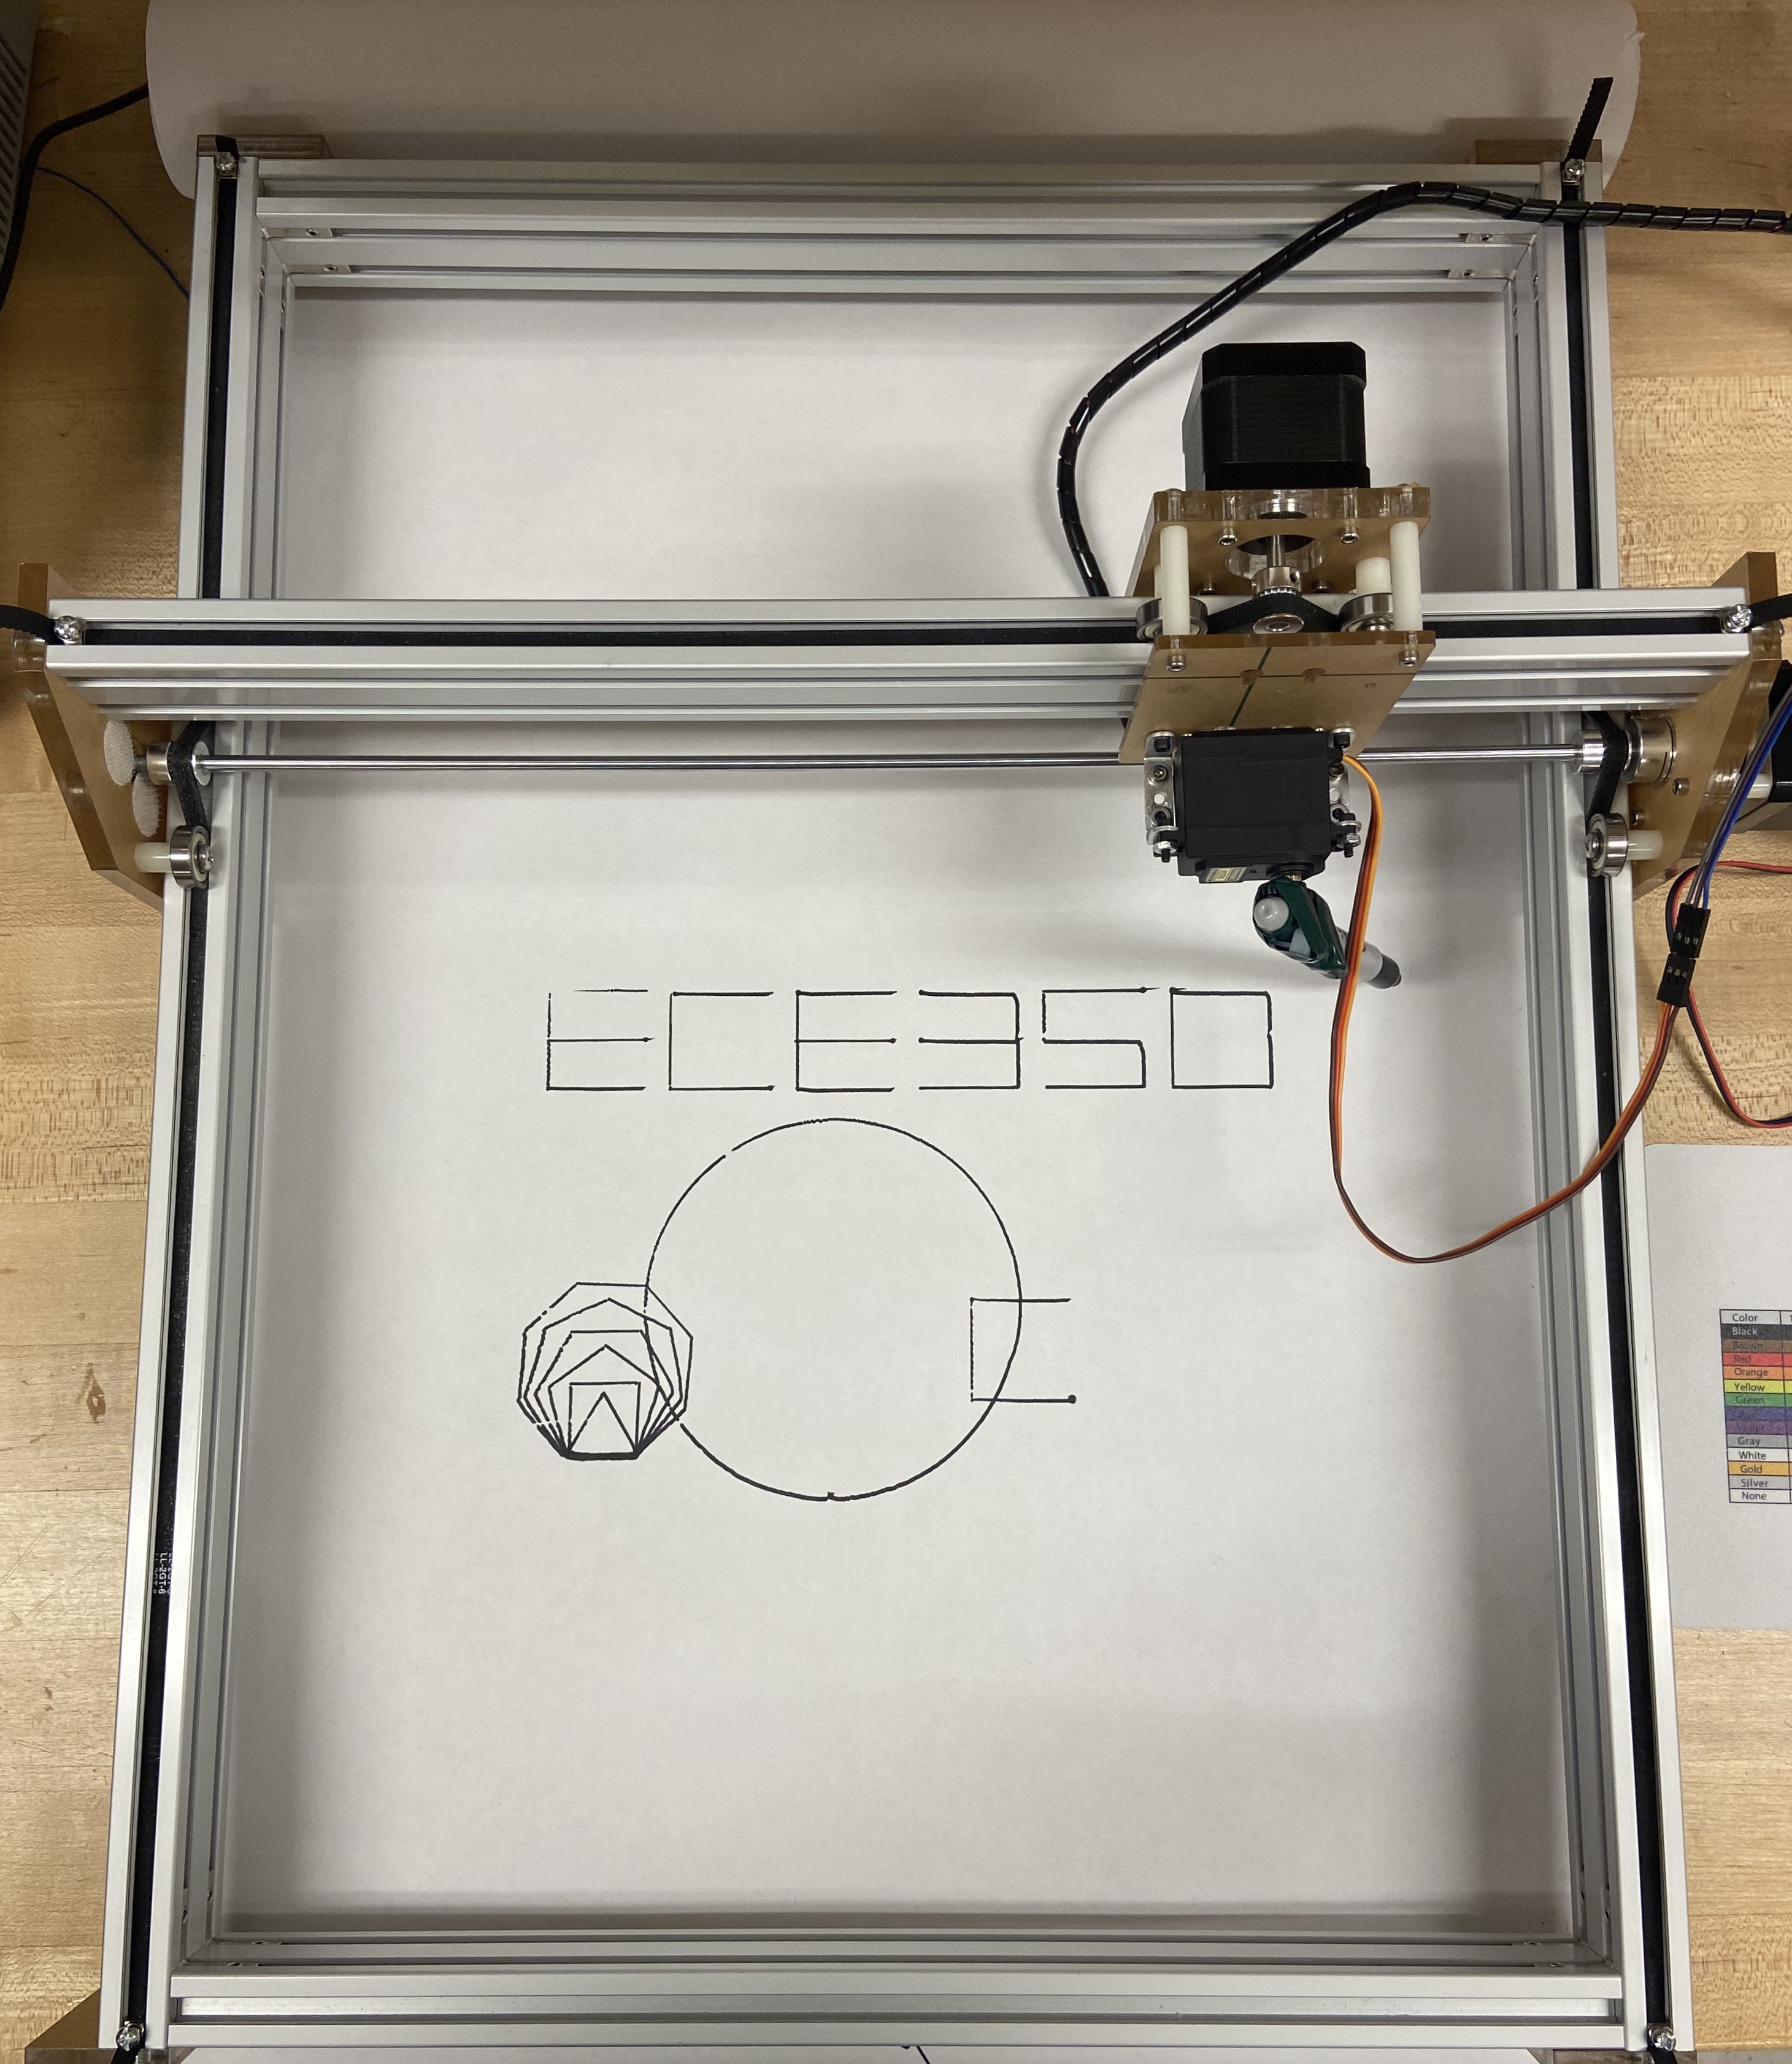
\includegraphics[width=0.9\textwidth]{IMG_0475.jpg}
\end{center}
\caption{Arial View with ECE350 Drawn}
\end{figure}

\section{Images}
\begin{figure}[ht!]
\begin{center}
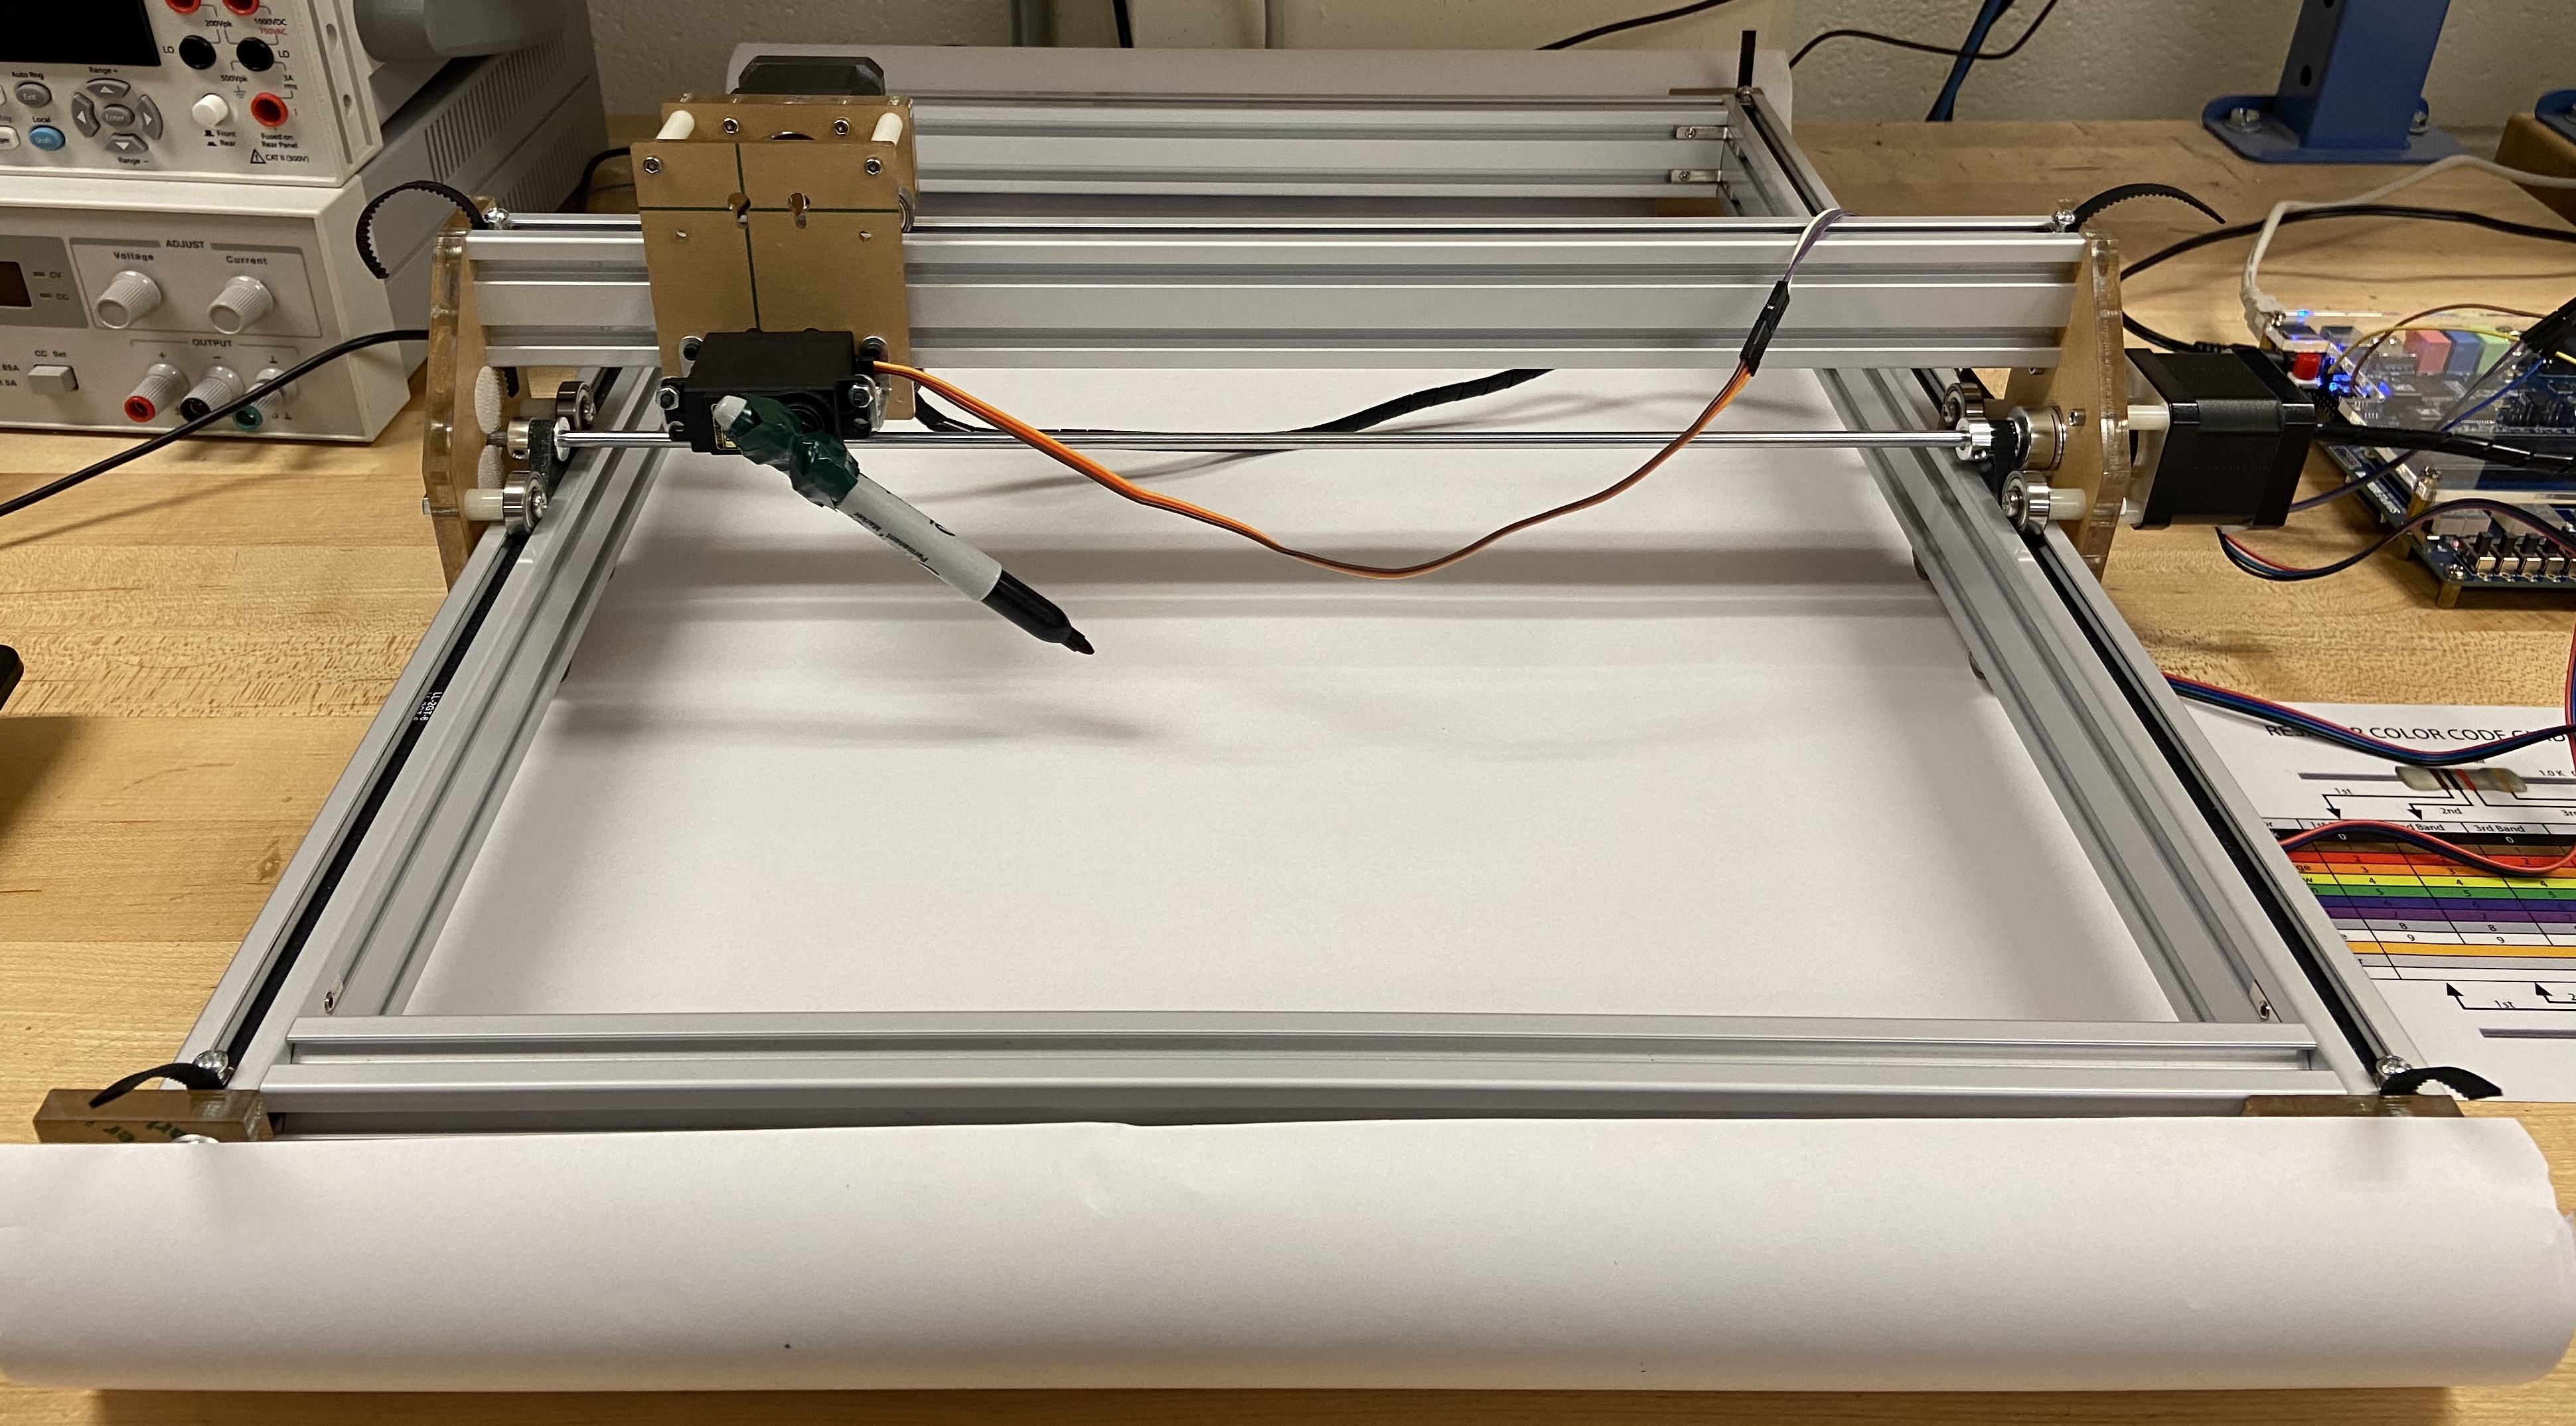
\includegraphics[width=0.9\textwidth]{IMG_0468.jpg}
\end{center}
\caption{Front View}
\end{figure}

\begin{figure}[ht!]
\begin{center}
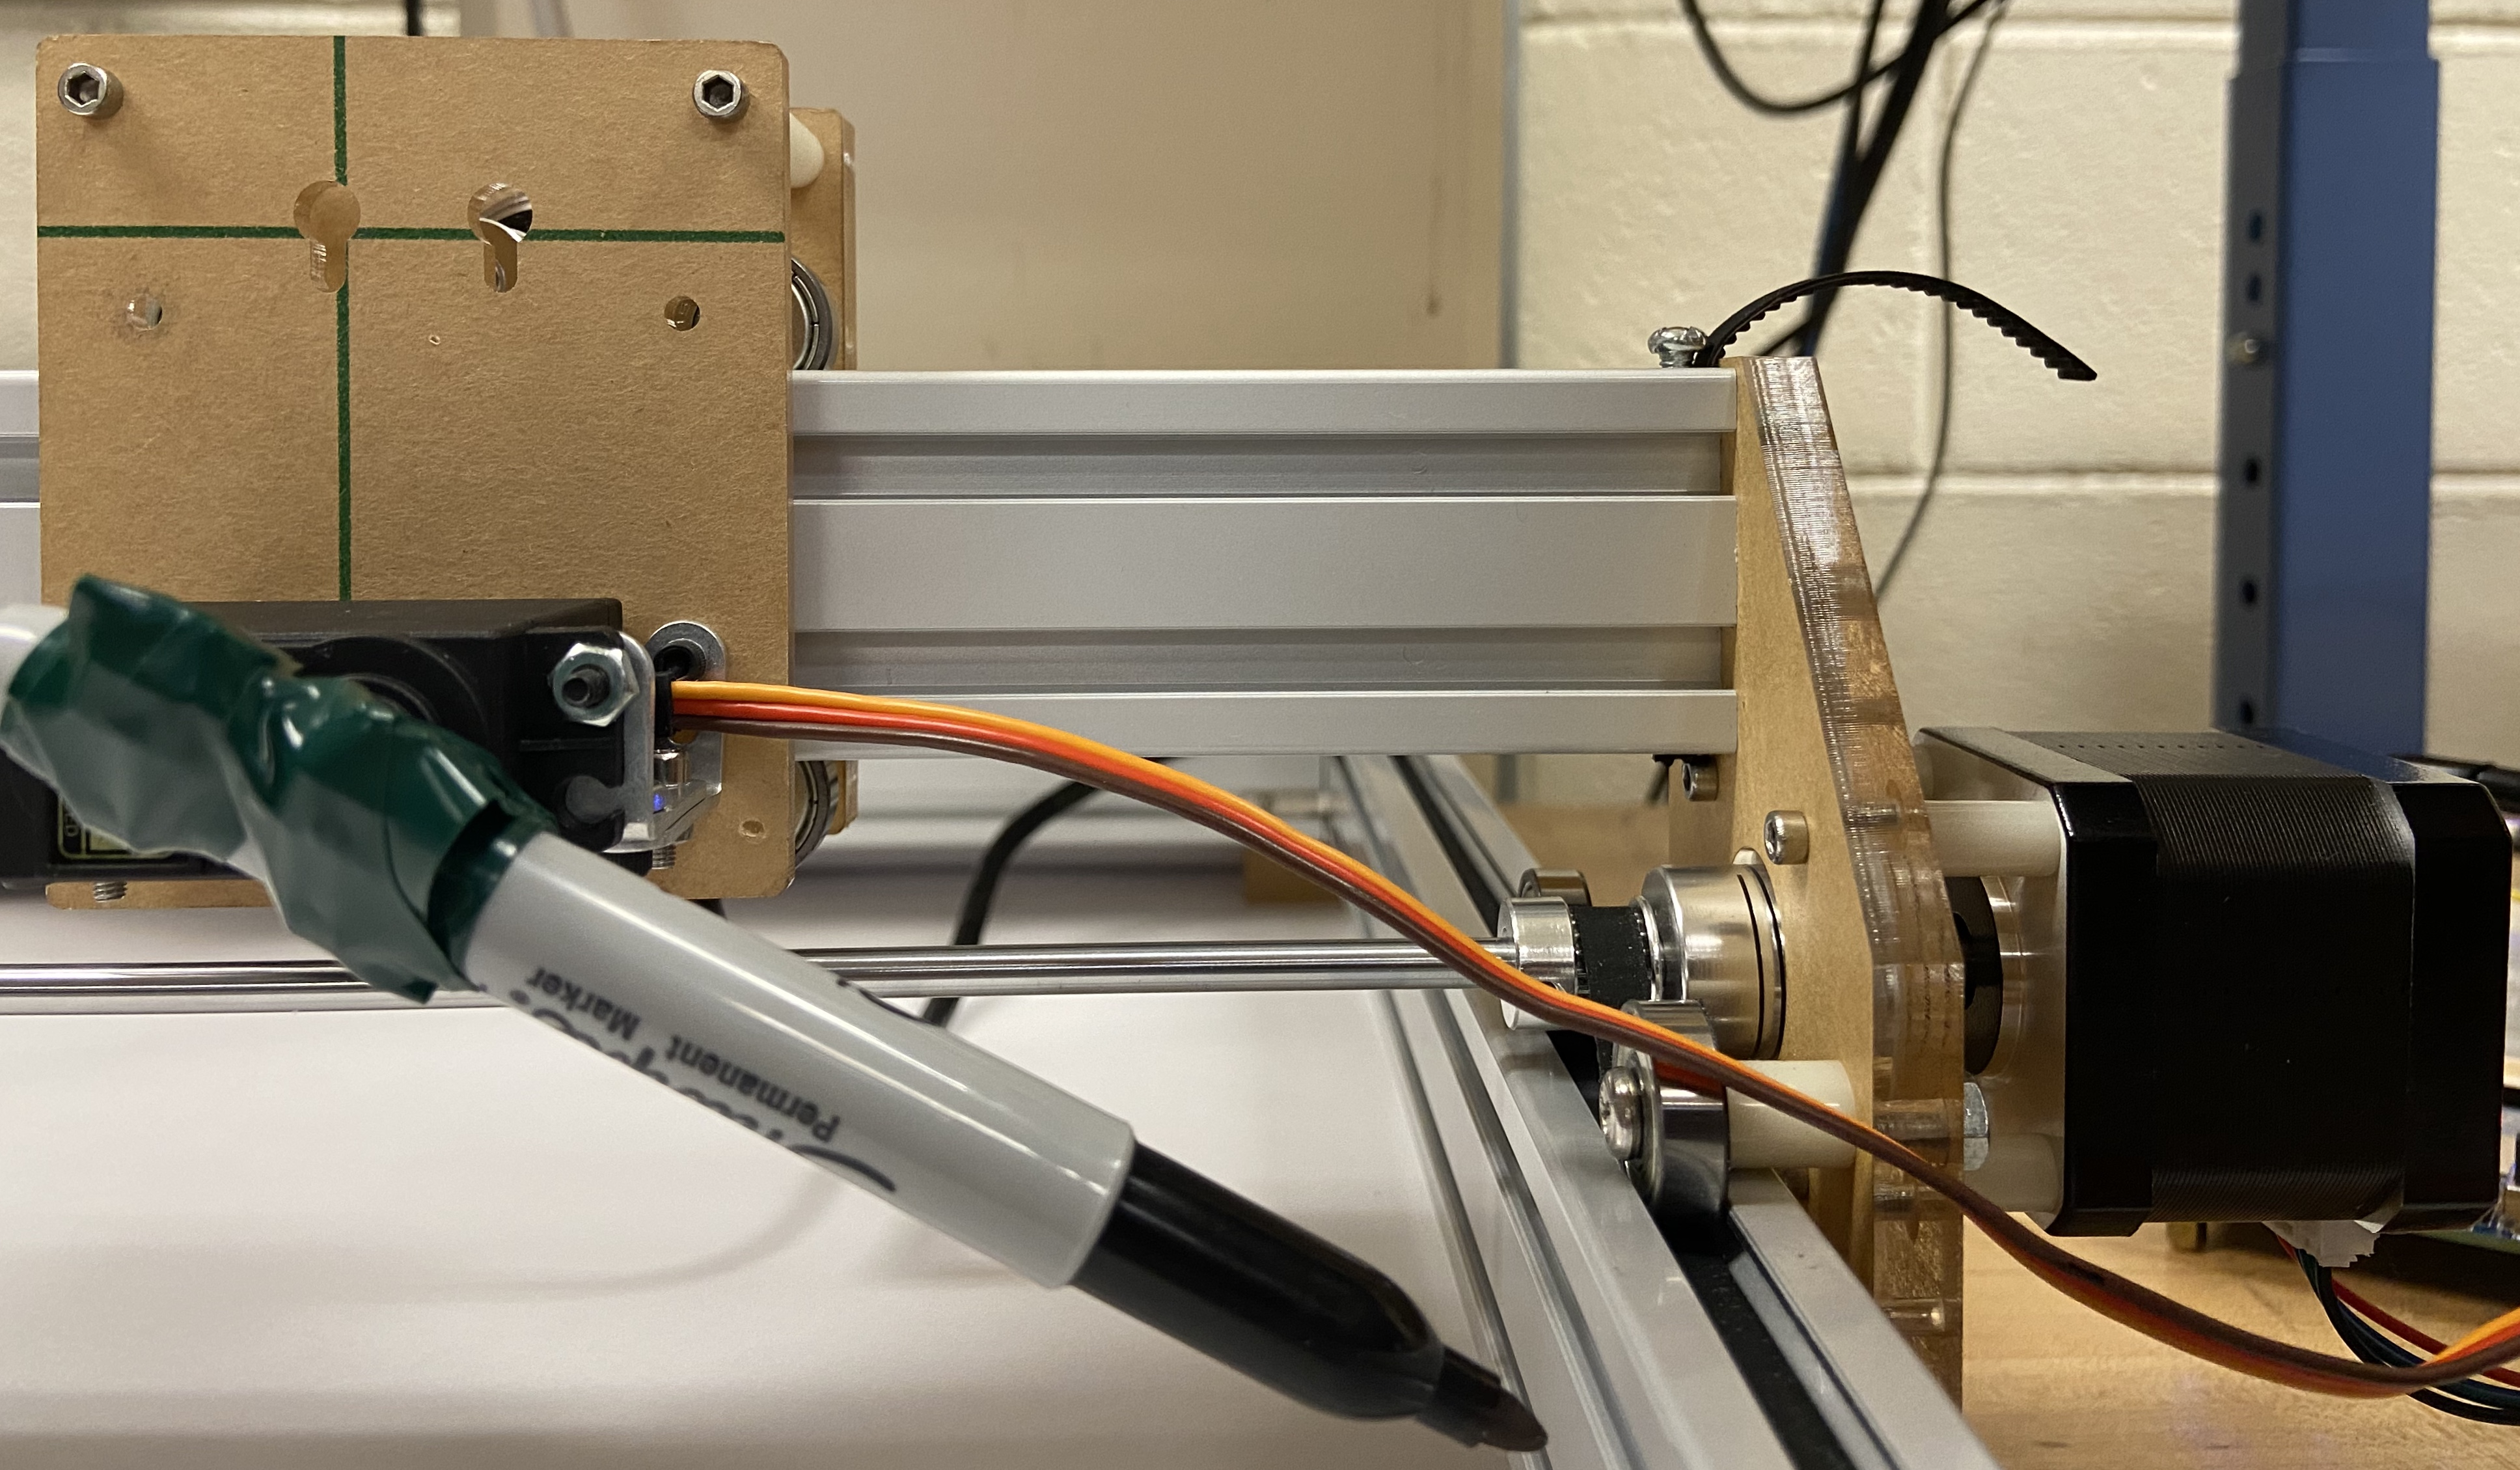
\includegraphics[width=0.9\textwidth]{IMG_0471.jpg}
\end{center}
\caption{Front View of Y-Axis Stepper Motor and Servo Motor}
\end{figure}

\begin{figure}[ht!]
\begin{center}
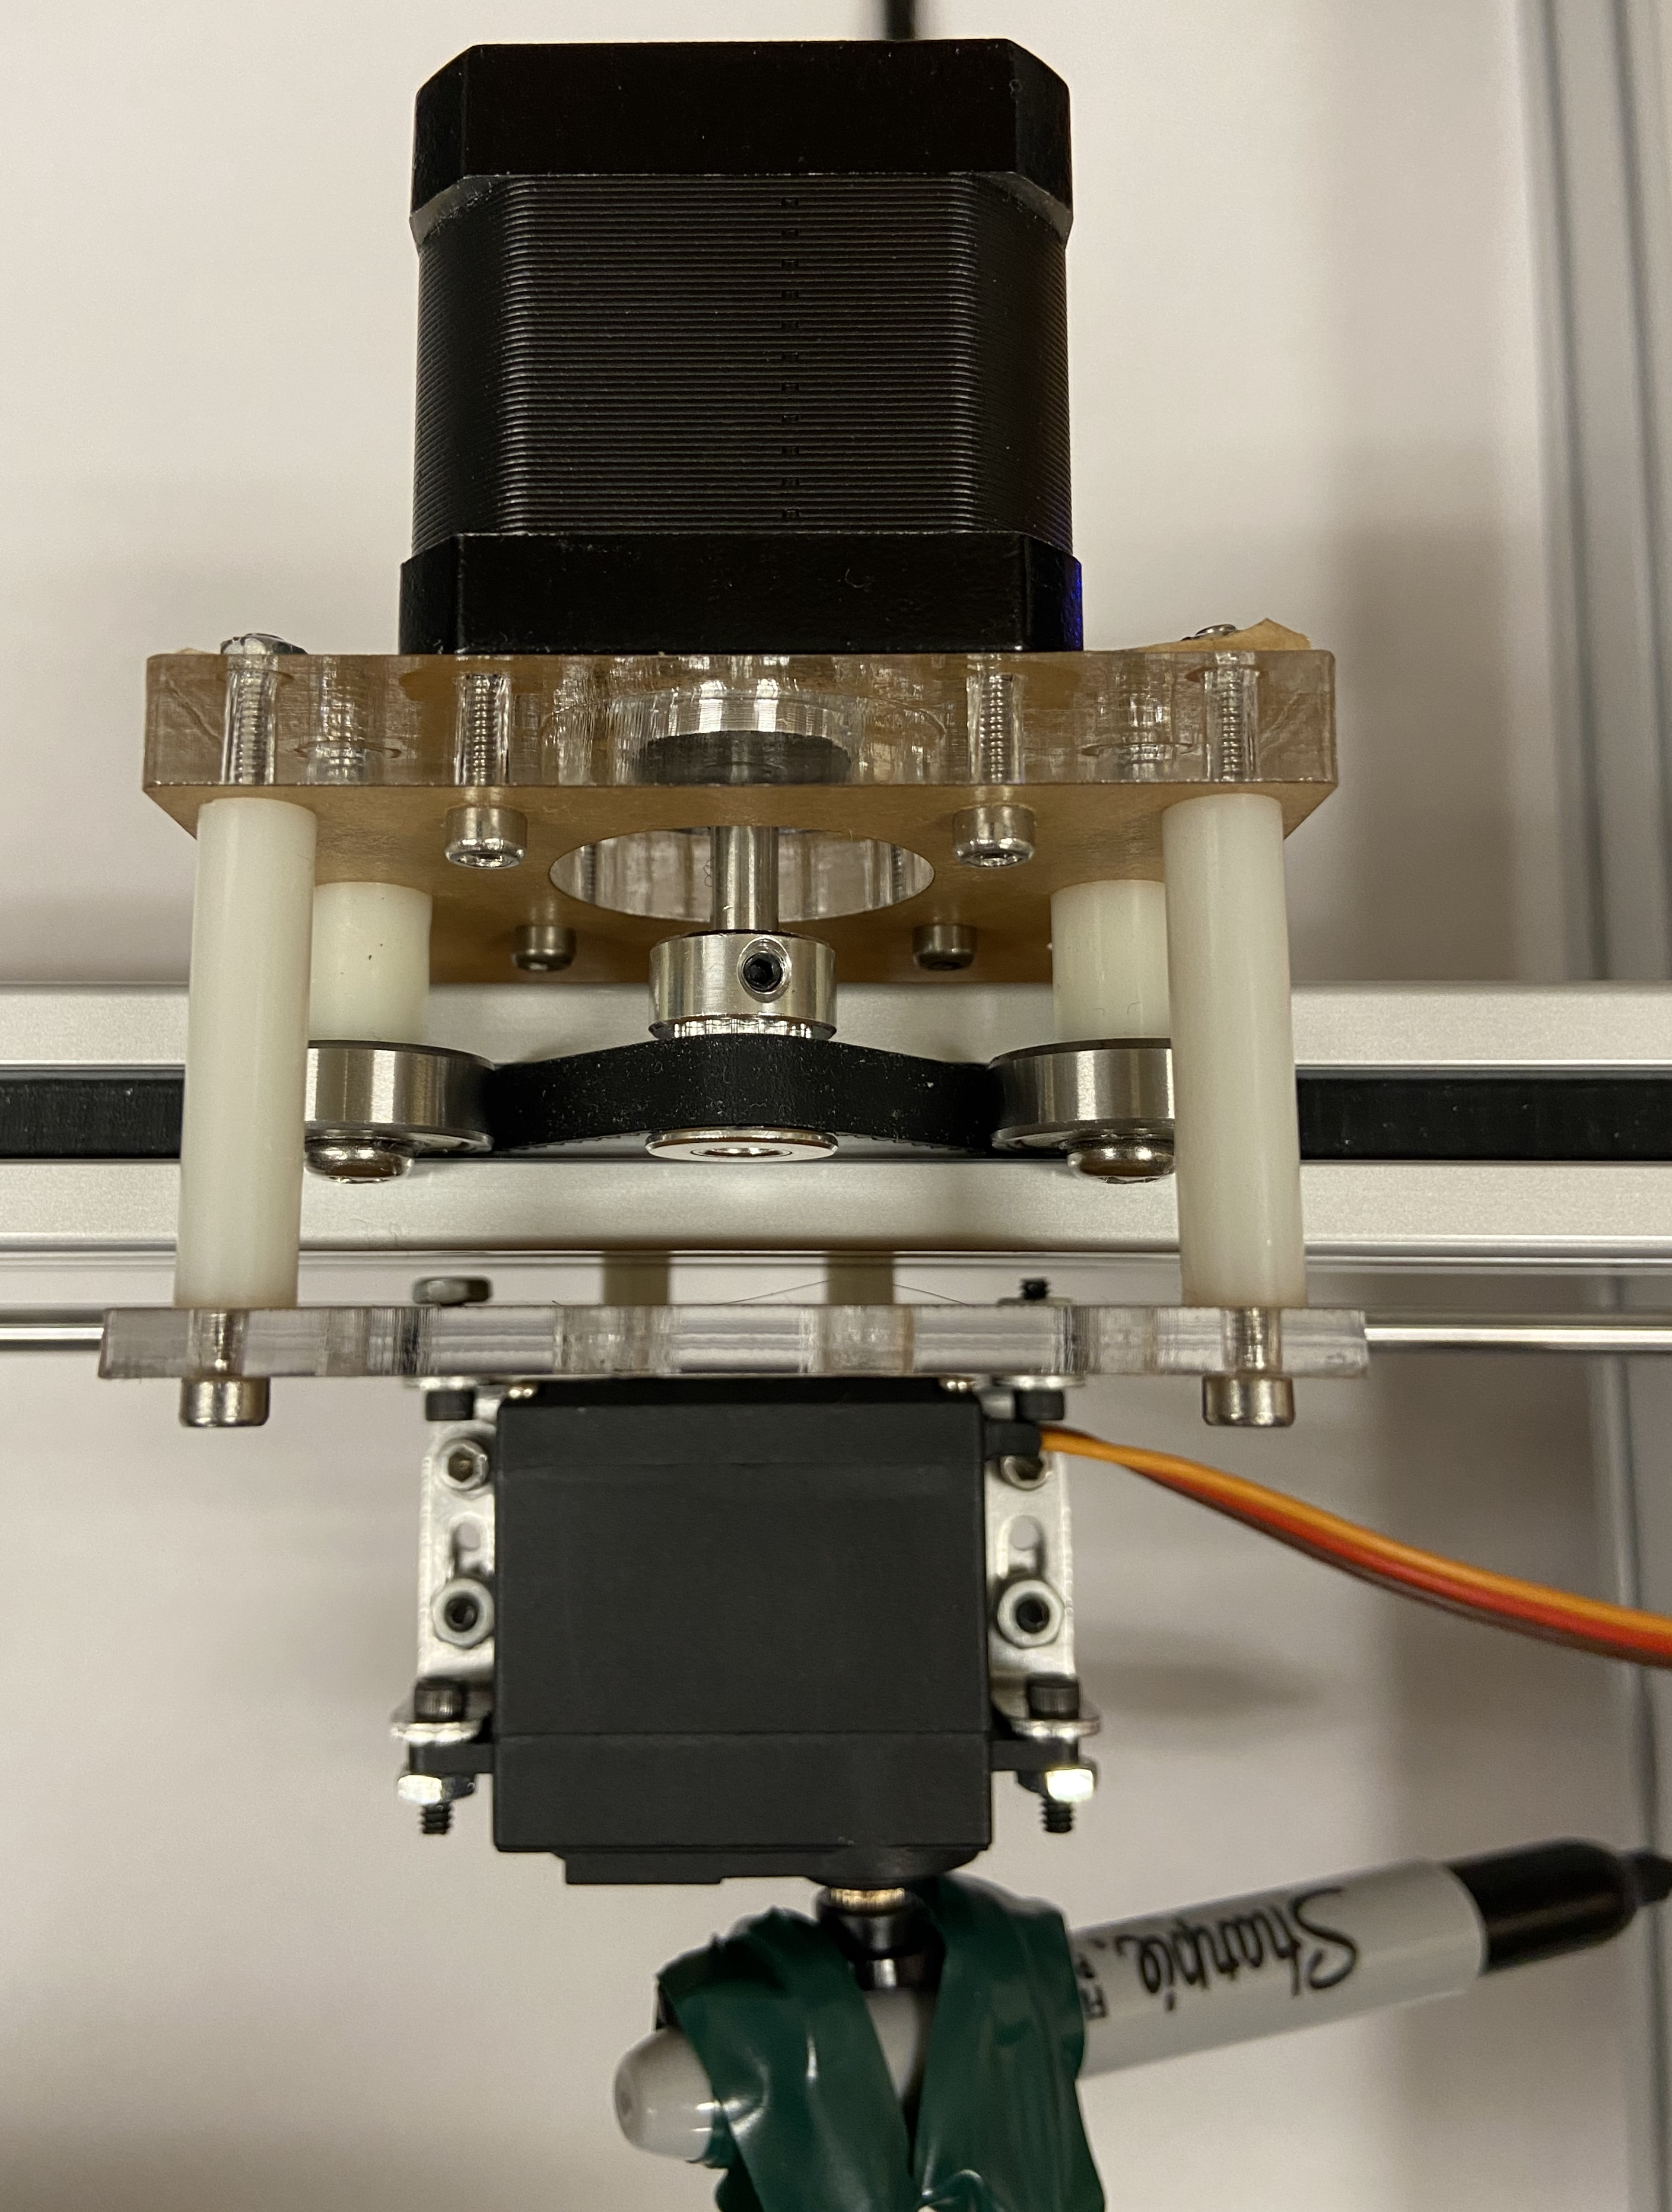
\includegraphics[width=0.9\textwidth]{IMG_0470.jpg}
\end{center}
\caption{Close Up of X-Axis Stepper Motor and Servo Motor}
\end{figure}

\end{document}
